\documentclass[11pt]{amsart}
\usepackage[T1]{fontenc}
\usepackage{lmodern}
\usepackage[margin=1.05in]{geometry}
\usepackage{amsmath,amssymb,mathtools}
\usepackage[expansion=false]{microtype}
\usepackage{enumitem}
\usepackage{xcolor}
\usepackage{tikz}
\usepackage[colorlinks=true,linkcolor=blue!45!black,citecolor=blue!45!black,
  urlcolor=blue!45!black]{hyperref}
\hypersetup{
 pdftitle={The affine Bernstein theorem in dimensions three through nine},
 pdfauthor={OpenAI},
 pdfsubject={Euclidean-complete affine maximal graphs},
 pdfkeywords={affine Bernstein conjecture, affine maximal hypersurface, convexity}
}
\pdfinfoomitdate=1
\pdftrailerid{}
\pdfsuppressptexinfo=15

\newcommand{\R}{\mathbb R}
\newcommand{\dd}{\mathop{}\!\mathrm d}
\DeclareMathOperator{\cof}{cof}
\DeclareMathOperator{\tr}{tr}
\newcommand{\Id}{\mathrm{Id}}
\newtheorem{theorem}{Theorem}[section]
\newtheorem{lemma}[theorem]{Lemma}
\newtheorem{proposition}[theorem]{Proposition}
\newtheorem{corollary}[theorem]{Corollary}
\theoremstyle{definition}
\newtheorem{definition}[theorem]{Definition}
\theoremstyle{remark}
\newtheorem{remark}[theorem]{Remark}
\numberwithin{equation}{section}
\setlist[itemize]{leftmargin=*,itemsep=3pt}
\setlist[enumerate]{leftmargin=*,itemsep=3pt}
\allowdisplaybreaks[1]

\title[The affine Bernstein theorem]{The affine Bernstein theorem\\
in dimensions three through nine}
\author{OpenAI}
\date{September 24, 2026}

\begin{document}

\begin{abstract}
We prove the Euclidean-complete affine Bernstein conjecture in dimensions
three through nine: a smooth locally uniformly convex affine maximal graph
is an elliptic paraboloid whenever its induced Euclidean metric is complete.
The same conclusion holds, without an initial graph assumption, for connected
smooth open (noncompact and without boundary) affine-complete locally uniformly
convex immersed hypersurfaces that are classically affine maximal in these
dimensions.
\end{abstract}

\maketitle

\section{Introduction}

The affine Bernstein problem asks whether a complete locally uniformly
convex affine maximal hypersurface must be an elliptic paraboloid.
The meaning of completeness is essential: completeness for the metric
induced from Euclidean space and completeness for the affine metric
are different hypotheses. We prove the Euclidean-complete graph
assertion in dimensions three through nine.

Let \(\Omega\subset\R^n\) be a nonempty open convex domain, and let
\(u\in C^\infty(\Omega)\) have positive-definite Hessian. Write
\[
 U^{ij}=\det(D^2u)(D^2u)^{-1}_{ij},
 \qquad
 w=(\det D^2u)^{-(n+1)/(n+2)}.
\]
The affine maximal equation is
\begin{equation}\label{eq:affine-maximal}
 U^{ij}w_{ij}=0.
\end{equation}
It is the Euler equation for affine area
\(\int(\det D^2u)^{1/(n+2)}\,\dd x\).

\begin{theorem}\label{thm:main}
Let \(3\le n\le9\). Suppose \(u\in C^\infty(\Omega)\) has
positive-definite Hessian and satisfies \eqref{eq:affine-maximal}.
If its graph is complete for the induced Euclidean metric
\[
 g_{ij}=\delta_{ij}+u_i u_j,
\]
then \(\Omega=\R^n\) and
\[
 u(x)=\tfrac12 x^{\mathsf T}Ax+b\cdot x+c
\]
for a positive-definite symmetric matrix \(A\), a vector \(b\), and a
constant \(c\). In particular, the graph is an invertible affine image
of the standard elliptic paraboloid.
\end{theorem}

Theorem~\ref{thm:main} resolves the Euclidean-complete affine Bernstein
conjecture for smooth locally uniformly convex graphs in dimensions
three through nine. It includes the entire graph assertion and
imposes neither a growth bound nor completeness of the affine metric.

Chern asked whether an entire locally uniformly convex affine maximal
surface must be an elliptic paraboloid \cite{Chern1979}.
Calabi developed the affine variational framework and proved the
surface conclusion under both Euclidean and affine completeness
\cite{Calabi1982}; see also \cite[Section~1]{TW2002}.
For a graph, the affine (Berwald--Blaschke) metric is
\[
 g^{\mathrm{aff}}_{ij}=(\det D^2u)^{-1/(n+2)}u_{ij},
\]
so its completeness is a different condition from that in
Theorem~\ref{thm:main}. Trudinger and Wang proved the
Euclidean-complete surface theorem, dispensing with affine
completeness \cite[Theorem~1.1]{TW2000}. Li and Jia gave a separate
proof of the surface theorem under affine completeness alone
\cite{LiJia2001}.

The analytic reduction in higher dimensions is also due to
Trudinger and Wang. Their interior estimates and rescaling argument
prove rigidity for Euclidean-complete graphs in every dimension provided
the separation of the graph
from its tangent planes has a modulus of strict convexity that remains
uniform under normalization of tangent-plane sublevel sets
\cite[Theorem~4.2 and Corollary~4.3]{TW2000}.
They establish this uniform control in dimension two by studying
convex limits and their supporting contact sets
\cite[Section~5]{TW2000}. Obtaining it in higher dimensions without
an additional hypothesis is the obstacle addressed here.
Later work has developed alternative analytic approaches: Wang and
Zhou give a proof of the entire-surface theorem using the partial
Legendre transform, and higher-dimensional rigidity results under
integral bounds on the Hessian and the inverse Hessian determinant
\cite[Theorem~1.2 and Corollary~1.6]{WangZhou2023}.
Our proof instead derives the required convexity control from the
geometry of affine limits, with no growth or integral bound assumed.

For locally uniformly convex hypersurfaces in dimension at least two,
Trudinger and Wang proved that affine completeness implies Euclidean
completeness
\cite[Theorem~A]{TW2002}; the converse fails in general.
Their global graph theorem \cite[Corollary~1]{TW2002} therefore extends
our conclusion to connected smooth open affine-complete locally
uniformly convex immersed hypersurfaces that are classically affine
maximal, without an initial graph assumption. The precise statement
and proof appear in Corollary~\ref{cor:affine-complete}.

The singular entire affine maximal graph constructed by Trudinger and
Wang in dimension ten \cite[Section~7]{TW2000} is a weak solution.
It is not smooth and does not furnish a counterexample under the
hypotheses of Theorem~\ref{thm:main}. Our argument identifies the
dimension restriction in a quadratic coercivity estimate, whose strict
positivity holds through dimension nine.

The distinction between the classical equation and its determinant-power
generalizations is also relevant. For affine maximal type equations
with \(w=(\det D^2u)^a\), Sun, Xing and Xu construct nonquadratic
Euclidean-complete examples in every dimension \(n\ge2\) for
\(a\in[-n/(n+1),0)\) \cite[Theorem~1.3]{SunXingXu2026}.
This interval excludes the classical exponent \(-(n+1)/(n+2)\)
in Equation~\eqref{eq:affine-maximal}.

\subsection*{The main ideas}
For \(a\in\Omega\), let
\[
 l_a(x)=u(a)+Du(a)\cdot(x-a),\qquad
 S_u(a,t)=\{x\in\Omega:u(x)<l_a(x)+t\}\quad(t>0).
\]
These tangent sections measure the separation of the graph from its
supporting planes. The geometric objective is uniform balance: for one
\(\rho>0\), reflection about the base point followed by contraction by
\(\rho\) takes every closed section into itself. This control must hold
at every base point and every height.

We obtain balance by studying full-dimensional closed convex limits of
affine images of the epigraph \(D=\{(x,z):x\in\Omega,\ z\ge u(x)\}\).
Write the coordinates of such a limit as
\((s,y)\in\R^k\times\R^{n+1-k}\). A model with \(k\) directions is
supported in \(s_i\ge0\), contains \(\{(s,0):s_i\ge0\}\), and has
compact caps cut out by \(\sum_i s_i\le T\). Its transverse fibers are
\(K_s=\{y:(s,y)\in D_{\mathrm{lim}}\}\), where \(D_{\mathrm{lim}}\)
denotes the limiting body. Maximizing \(k\) forces a uniform centering
estimate \(-K_s\subset C_*K_s\) for all positive fibers: failure of
this estimate produces an additional nonnegative direction by a further
affine rescaling. Normalized caps and convex limits also play a central
role in the two-dimensional argument of Trudinger and Wang
\cite[Section~5]{TW2000}; here the rescaling is organized by the maximal
number of nonnegative directions.

The analytic step excludes \(k\ge2\). Support functions of the fibers
give a positive second form and a natural invariant measure. The
affine maximal equation yields an integral inequality in logarithmic
coordinates, forcing exponential growth of a related measure.
A cap identity and estimates for Hessian minors bound its mass on
each normalized log cell, allowing only polynomial growth.
Both estimates are used on smooth approximants over one sufficiently
large finite box; the limiting body needs no regularity.

These two ingredients---increasing the number of model directions
when centering degenerates, and combining a logarithmic integral
inequality with affine-invariant cell bounds---are the principal
technical contributions. The resulting uniform balance of tangent
sections supplies a scale-independent modulus of strict convexity.
We then use the interior estimates and section-rescaling argument of
Trudinger and Wang \cite[Sections~2 and~4]{TW2000}: normalized third
derivatives stay bounded, while transforming them back gives a bound
tending to zero. John's ellipsoid theorem \cite{John1948,Ball1992}
supplies the normalizations. The compactness arguments and the cap and
tube estimates used here are proved below.

\subsection*{Notation and organization}
Closed sections use the corresponding non-strict inequality.
The symbol \(B_r(x)\) denotes an open Euclidean ball, and \(B_r=B_r(0)\);
its ambient dimension will be clear. The notation \(H^{-1}\)
for a positive second form specifies the dual norm on covectors.
All constants in uniform estimates may depend on the fixed dimension
and, where stated, on the family of affine limits of the given
epigraph.

Section~\ref{sec:geometry} establishes the compactness and centering
argument. Sections~\ref{sec:area} and \ref{sec:tubes} derive the cap
identity and the tube inequality. Section~\ref{sec:bounds} excludes
models with several directions, and Section~\ref{sec:rigidity}
deduces section control and proves Theorem~\ref{thm:main}.

\section{Convex limits and centered fibers}\label{sec:geometry}

The objective of this section is to show that fibers are uniformly
centered once the number of model directions is maximal. We first
obtain compact caps from graph completeness, then normalize a hypothetical
sequence of increasingly asymmetric fibers. Its limit supplies the
additional direction that contradicts maximality.

Throughout this section, $n\ge2$, $\Omega\subset\R^n$ is nonempty,
open and convex, and $u\in C^\infty(\Omega)$ has positive-definite Hessian.
We assume only that its graph is complete for the induced Euclidean
metric.  No differential equation is needed in this section.
For $a\in\Omega$, write
\[
 l_a(x)=u(a)+Du(a)\cdot(x-a),
 \qquad g_a(x)=u(x)-l_a(x).
\]

\begin{lemma}\label{lem:proper-sections}
At every finite boundary point $b\in\partial\Omega$,
\[
 \lim_{\Omega\ni x\to b}u(x)=+\infty.
\]
The epigraph
\[
 D=\{(x,z):x\in\Omega,\ z\ge u(x)\}
\]
is a closed full-dimensional convex set with boundary equal to the
graph of $u$.  For every $a\in\Omega$ and $t\ge0$, the set
$\{x\in\Omega:g_a(x)\le t\}$ is compact and contained in $\Omega$.
Consequently the cap $D\cap\{z-l_a(x)\le t\}$ is compact.
\end{lemma}

\begin{proof}
Suppose $x_j\to b\in\partial\Omega$ and $u(x_j)\le A$.
Fix $a\in\Omega$.  Convexity, followed by continuity at the interior
point $a+q(b-a)$, gives
\[
 u(a+q(b-a))\le (1-q)u(a)+qA,\qquad 0\le q<1.
\]
An affine supporting function at $a$ gives a lower bound on the same
segment.  The resulting bounded convex function of $q$ has finite
total variation and a finite limit as $q\uparrow1$.  Its lifted curve
has finite Euclidean length, since
\[
 \int_0^1\sqrt{|b-a|^2+
       \left|\frac{\dd}{\dd q}u(a+q(b-a))\right|^2}\,\dd q
 \le |b-a|+\int_0^1
       \left|\frac{\dd}{\dd q}u(a+q(b-a))\right|\,\dd q<\infty.
\]
Its tail is therefore Cauchy in the graph metric, but its base
coordinate tends to $b\notin\Omega$.  This contradicts completeness.
The asserted boundary limit follows.  It also shows that a bounded
convergent sequence of points of $D$ cannot have its base limit on
$\partial\Omega$.  Thus $D$ is closed, and its boundary is exactly
the graph.

Choose $r,c>0$ such that $\overline B_r(a)\subset\Omega$ and
$D^2u\ge c\Id$ on this ball.  Along every ray from $a$, convexity of
$g_a$, together with $g_a(a)=0$, gives
\[
 g_a(x)\ge \frac{cr}{2}|x-a|
 \qquad (x\in\Omega,\ |x-a|\ge r).
\]
Indeed, $g_a\ge cr^2/2$ at the point of the ray at distance $r$,
and its quotient by the distance is nondecreasing.  Thus each stated
sublevel is bounded.  The boundary limit just proved makes it closed
in $\R^n$ and contained in $\Omega$.  On such a compact base, both
$l_a$ and the cap height are bounded, which proves the last claim.
\end{proof}

We use local convergence of nonempty closed convex sets in the sense
of locally uniform convergence of their distance functions.
This topology has the following elementary properties.  Every point
of a limit is approximated by points of the approximating sets, and
every limit of a convergent sequence of such points belongs to the
limit.  If the limit has nonempty interior, every compact subset of
its interior is eventually contained in the interiors of the
approximants.  For the latter statement, enclose a point in a simplex
whose vertices lie in the limit, approximate its vertices, and then
use a finite cover of the compact subset.  A sequence of closed convex
sets meeting a fixed bounded set has a locally convergent subsequence:
their distance functions are locally equibounded and $1$-Lipschitz,
and a diagonal application of compactness gives the distance function
of a nonempty closed convex set.

Let $\mathcal F(D)$ be the family of all full-dimensional local
limits of invertible affine images of $D$, including those images
themselves.  The family is invariant under invertible affine maps
and closed under further full-dimensional local limits.  To justify
the last assertion explicitly, the distance-function topology is
metrizable by
\[
 d_{\mathrm{loc}}(C,E)=
 \sum_{q=1}^{\infty}2^{-q}
 \min\left\{1,\sup_{|X|\le q}
       |\operatorname{dist}(X,C)-\operatorname{dist}(X,E)|\right\}.
\]
If $C_j\in\mathcal F(D)$ tends to a full-dimensional set $C$, choose
an affine image $E_j$ of $D$ with
$d_{\mathrm{loc}}(E_j,C_j)<1/j$.  Then $E_j\to C$.
Affine invariance follows because a fixed invertible affine map and
its inverse take bounded sets to bounded sets and preserve the two
pointwise convergence properties above.  Thus affine maps varying
with $j$ may be applied before this diagonal choice.

\begin{lemma}\label{lem:cap-compactness}
Suppose $C_j\to C$ locally, and let $\ell$ be an affine function.
If $C\cap\{\ell\le b\}$ is bounded and contains a point $q$ with
$\ell(q)<b$, then the caps $C_j\cap\{\ell\le b\}$ are eventually
uniformly bounded.  They converge in Hausdorff distance to
$C\cap\{\ell\le b\}$.
\end{lemma}

\begin{proof}
Choose $q_j\in C_j$ with $q_j\to q$, so $\ell(q_j)<b$ eventually.
If points $p_j\in C_j\cap\{\ell\le b\}$ escape every bounded set,
pass to a subsequence for which
\[
 \frac{p_j-q_j}{|p_j-q_j|}\longrightarrow v,\qquad |v|=1.
\]
For each fixed $t\ge0$, the points
$q_j+t(p_j-q_j)/|p_j-q_j|$ eventually lie on the segments
$[q_j,p_j]$.  Their limit $q+tv$ therefore belongs to
$C\cap\{\ell\le b\}$, contradicting boundedness.

Uniform boundedness and local convergence show that every limit
point of the approximating caps lies in the limit cap.  Conversely,
if $x$ belongs to the limit cap, then
$(1-\eta)x+\eta q$ lies strictly below the top for every
$0<\eta\le1$ and is approximated by points of the approximating
caps.  Letting $\eta\downarrow0$ and using compactness gives the
reverse Hausdorff inclusion.
\end{proof}

\begin{definition}\label{def:model}
A \emph{model with $k$ directions}, or a \emph{$k$-model}, is a member
$C$ of $\mathcal F(D)$ equipped with affine coordinates
\[
 (s,y)\in\R^k\times\R^m,\qquad m=n+1-k,
 \qquad 1\le k\le n+1,
\]
such that
\[
 \{(s,0):s_i\ge0\}\subset C
 \subset\{(s,y):s_i\ge0\},
\]
and every cap $C\cap\{\sum_i s_i\le T\}$, $T\ge0$, is compact.
Its transverse fibers are
\[
 K_s=\{y:(s,y)\in C\}.
\]
The coordinates are part of the model data.
\end{definition}

\begin{lemma}\label{lem:model-fibers}
For a $k$-model, addition of any vector $(v,0)$ with $v_i\ge0$
preserves $C$.  Every fiber $K_s$ with $s_i>0$ is compact,
full-dimensional in $\R^m$, and contains zero.  Moreover,
\begin{equation}\label{eq:fiber-monotonicity}
 K_s\subset K_t\quad(s_i\le t_i),
 \qquad K_{\lambda s}\subset\lambda K_s\quad(\lambda\ge1).
\end{equation}
At least one $1$-model exists.
\end{lemma}

\begin{proof}
The recession assertion holds for any closed convex set containing
the indicated orthant, without a full-dimensionality assumption.
For $X\in C$ and $v_i\ge0$, take the limit as $\eta\downarrow0$ of
\[
 (1-\eta)X+\eta(v/\eta,0)\in C
\]
to obtain $X+(v,0)\in C$.  This proves fiber monotonicity.
Since the ambient origin belongs to $C$, contraction toward it
proves the second inclusion in \eqref{eq:fiber-monotonicity}.
Containment of zero and compactness follow from the definition.

Take an interior ball of $C$ centered at $(s^0,y^0)$; all coordinates
of $s^0$ are positive.  Given $s_i>0$, choose $0<\eta\le1$ with
$\eta s^0_i\le s_i$.  Contract the transverse slice of this ball
by $\eta$ about the ambient origin, and increase the $s$ coordinates
to $s$.  The resulting transverse ball lies in $K_s$, proving full
dimension.  When $m=0$ this assertion uses the usual convention for
$\R^0$.

Finally, for any $a\in\Omega$, the coordinates
$s=z-l_a(x)$ and $y=x-a$ make $D$ a $1$-model by
Lemma~\ref{lem:proper-sections}.
\end{proof}

We shall use the following precise consequence of the ellipsoid
theorem of John~\cite{John1948}; see also the contact-point formulation
and nonsymmetric outer-radius deduction in \cite[Section~0]{Ball1992}.
The normalization is linear and
therefore preserves the distinguished origin.

\begin{lemma}\label{lem:linear-normalization}
Let $K\subset\R^d$, $d\ge1$, be compact and convex with nonempty
interior and $0\in K$.  There are an invertible linear map $A$ and
a vector $c$ such that
\begin{equation}\label{eq:linear-normalization}
 \overline B_1(c)\subset AK\subset\overline B_d(c),
 \qquad |c|\le d.
\end{equation}
In particular $AK\subset\overline B_{2d}$; the origin is allowed
to lie on $\partial K$.
If in addition $-K\subset C_*K$ for some $C_*\ge1$, then
\begin{equation}\label{eq:centered-normalization}
 \overline B_{2/(C_*+1)}
 \subset AK\subset\overline B_{2d}.
\end{equation}
\end{lemma}

\begin{proof}
Choose a maximum-volume inscribed ellipsoid and take the linear
part of its normalization to a unit ball.  John's Theorem gives
the two inclusions in \eqref{eq:linear-normalization}.  Since
$0\in AK$, the outer inclusion implies $|c|\le d$.
The centering assumption also gives
$\overline B_{1/C_*}(-c/C_*)\subset AK$.  The convex combination of
this ball and $\overline B_1(c)$ with respective weights
$C_*/(C_*+1)$ and $1/(C_*+1)$ is the centered ball in
\eqref{eq:centered-normalization}.
\end{proof}

By Lemma~\ref{lem:model-fibers}, the set of direction numbers achieved
by models is a nonempty subset of $\{1,\ldots,n+1\}$.  Let $k$ be
its maximum.

\begin{proposition}[Uniform centering at maximal direction number]
\label{prop:centering}
Suppose $m=n+1-k>0$.  There is a constant $C_*\ge1$, depending on
the family $\mathcal F(D)$, such that
\begin{equation}\label{eq:model-centering}
 -K_s\subset C_*K_s
 \qquad(s_i>0)
\end{equation}
for every $k$-model and every admissible choice of its coordinates.
In particular, zero is an interior point of every such fiber.
\end{proposition}

\begin{proof}
Suppose that no uniform constant exists.  Choose $k$-models and
positive fibers for which the inclusion with constant $j$ fails.
Positive diagonal changes in $s$ put those fibers at
$\mathbf1=(1,\ldots,1)$, and Lemma~\ref{lem:linear-normalization}
provides linear changes in $y$.  Denote the resulting models by
$C_j$ and their fibers at $\mathbf1$ by $F_j$.  Thus
\begin{equation}\label{eq:asymmetric-normalization}
 \overline B_1(c_j)\subset F_j\subset\overline B_{2m},
 \qquad |c_j|\le m,
 \qquad -F_j\not\subset jF_j.
\end{equation}
All these coordinate changes preserve the model properties and
the failed inclusion.

For $T\ge1$ and $0\le s_i\le T$,
Lemma~\ref{lem:model-fibers} gives
\begin{equation}\label{eq:normalized-cap-bound}
 K_s^{(j)}\subset K_{T\mathbf1}^{(j)}
 \subset T F_j\subset\overline B_{2mT}.
\end{equation}
Pass to a local limit $C$ and a subsequence with $c_j\to c$.
The limit is contained in the nonnegative $s$ halfspaces, contains
the entire orthant at $y=0$, and has compact caps by
\eqref{eq:normalized-cap-bound}.  Moreover,
\[
 [1,2]^k\times\overline B_1(c_j)\subset C_j,
\]
so its limit has nonempty interior.  The closure properties of
$\mathcal F(D)$ show that $C$ is a $k$-model.

Its fiber $F=K_{\mathbf1}$ is the Hausdorff limit of $F_j$.
Only one inclusion needs explanation.  If
$(s^{(j)},y_j)\in C_j$ tends to $(\mathbf1,y)\in C$, let
\[
 a_j=\min\left\{1,\frac1{s^{(j)}_1},\ldots,
                         \frac1{s^{(j)}_k}\right\}.
\]
The denominators are positive for large $j$, and $a_j\to1$.
Contracting by $a_j$ and then increasing the $s$ coordinates gives
$(\mathbf1,a_jy_j)\in C_j$.  Thus every point of $F$ is approximated
from the exact fibers $F_j$; the other inclusion follows from local
convergence.  Uniform boundedness makes this Hausdorff convergence.
If zero were interior to $F$, the $F_j$ would eventually contain a
fixed ball centered at zero.  Their common outer bound would then
give a fixed centering constant, contrary to
\eqref{eq:asymmetric-normalization}.  Hence $0\in\partial F$.

A supporting linear functional of $F$ at zero can be made the
coordinate $y_1$, with $F\subset\{y_1\ge0\}$.  This inequality
holds on all of $C$: contract any $(s,y)\in C$ until each $s_i\le1$,
then increase the $s$ coordinates to $\mathbf1$ and apply the
inequality on $F$.  Since $F$ has nonempty interior, an additional
invertible linear choice of transverse coordinates makes an
interior point of $F$ equal to $(y_1,y')=(1,0)$, while retaining
the global support $y_1\ge0$.

We now construct a model with $k+1$ directions.  Put $d=m-1$.
For $0<\epsilon<1/2$, let
\[
 F_\epsilon=
 \{y'\in\R^d:(\mathbf1,\epsilon,y')\in C\}.
\]
This compact slice contains zero in its interior when $d>0$.
Indeed, if $\overline B_r((1,0))\subset F$, contracting by
$\epsilon$ about the ambient origin and then adding
$(1-\epsilon)\mathbf1$ in the $s$ coordinates shows that
\[
 \overline B_{\epsilon r}\subset F_\epsilon\subset\R^d.
\]
When $d>0$, apply Lemma~\ref{lem:linear-normalization} to choose an invertible
linear map $A_\epsilon$ on $\R^d$ so that
\[
 \overline B_1(c_\epsilon)\subset A_\epsilon F_\epsilon
 \subset\overline B_{2d},\qquad |c_\epsilon|\le d.
\]
If $d=0$, take $A_\epsilon$ to be the unique linear automorphism of
$\R^0$ and omit all statements about its balls.
Use the affine images
\[
 C_\epsilon=
 \{(s,r,z):(s,\epsilon r,A_\epsilon^{-1}z)\in C\}.
\]
They are supported in $s_i,r\ge0$, contain the origin, and their
slice at $(s,r)=(\mathbf1,1)$ has the stated normalization.

Figure~\ref{fig:thin-slice} illustrates the supporting fiber and the
slice used in this rescaling. The remaining step is to turn control of
that one slice into a uniform bound for every fixed cap.
\begin{figure}[tbp]
\centering
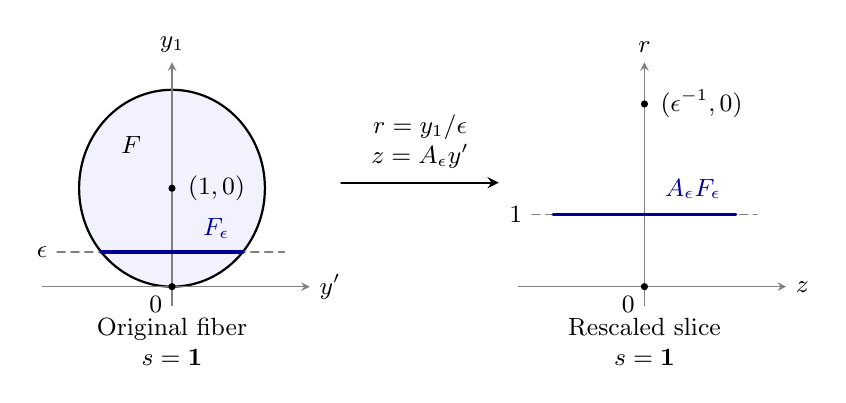
\begin{tikzpicture}[x=1cm,y=1cm,>=stealth,
  every node/.style={font=\small},line cap=round]
  \begin{scope}[shift={(0,0)}]
    \fill[blue!5] (0,1.25) ellipse[x radius=1.18,y radius=1.25];
    \draw[thick] (0,1.25) ellipse[x radius=1.18,y radius=1.25];
    \draw[->,gray] (-1.65,0)--(1.75,0) node[right,black] {$y'$};
    \draw[->,gray] (0,-.24)--(0,2.85) node[above,black] {$y_1$};
    \draw[densely dashed,gray] (-1.46,.44)--(1.43,.44);
    \draw[very thick,blue!60!black] (-.899,.44)--(.899,.44);
    \node[left] at (-1.46,.44) {$\epsilon$};
    \node[anchor=south west,blue!60!black] at (.27,.49) {$F_\epsilon$};
    \fill (0,0) circle[radius=1.3pt];
    \node[below left] at (0,0) {$0$};
    \fill (0,1.25) circle[radius=1.3pt];
    \node[anchor=west] at (.08,1.25) {$(1,0)$};
    \node at (-.52,1.8) {$F$};
    \node[align=center] at (0,-.7) {Original fiber\\$s=\mathbf1$};
  \end{scope}
  \draw[->,thick] (2.15,1.32)--(4.15,1.32);
  \node[align=center] at (3.15,1.84)
    {$r=y_1/\epsilon$\\$z=A_\epsilon y'$};
  \begin{scope}[shift={(6,0)}]
    \draw[->,gray] (-1.6,0)--(1.8,0) node[right,black] {$z$};
    \draw[->,gray] (0,-.24)--(0,2.85) node[above,black] {$r$};
    \draw[densely dashed,gray] (-1.43,.92)--(1.43,.92);
    \draw[very thick,blue!60!black] (-1.16,.92)--(1.16,.92);
    \node[left] at (-1.43,.92) {$1$};
    \node[anchor=south west,blue!60!black] at (.14,.99)
      {$A_\epsilon F_\epsilon$};
    \fill (0,0) circle[radius=1.3pt];
    \node[below left] at (0,0) {$0$};
    \fill (0,2.32) circle[radius=1.3pt];
    \node[anchor=west] at (.08,2.32) {$(\epsilon^{-1},0)$};
    \node[align=center] at (0,-.7) {Rescaled slice\\$s=\mathbf1$};
  \end{scope}
\end{tikzpicture}
\caption{The change from $(y_1,y')$ to $(r,z)$ at the fixed base
point $s=\mathbf1$, shown schematically with one $y'$ coordinate.
The actual fiber need not have the smooth or symmetric shape drawn here.
The slice $y_1=\epsilon$ becomes the slice $r=1$, while
$A_\epsilon$ normalizes its remaining transverse coordinates.
The interior point $(1,0)$ of $F$ is sent to
$(\epsilon^{-1},0)$. The right panel shows only this point, the
origin, and the distinguished slice; the shape of the transformed
fiber is omitted.}
\label{fig:thin-slice}
\end{figure}


Here is a uniform bound for their caps.  Suppose
$(s,r,z)\in C_\epsilon$ with $s_i,r\le T$, where $T\ge1$.
Increase $s$ to $T\mathbf1$ and contract by $1/T$.  This gives
\[
 (\mathbf1,q,z/T)\in C_\epsilon,
 \qquad q=r/T\in[0,1].
\]
The point $(\mathbf1,2,0)$ also belongs to $C_\epsilon$, since
$2\epsilon<1$ and it is obtained by contracting
$(\mathbf1,1,0)\in C$ and then increasing $s$.
Interpolate these two points with weight
\[
 a=\frac1{2-q}\in[1/2,1]
\]
on $(\mathbf1,q,z/T)$.  The resulting point is
$(\mathbf1,1,az/T)$, so the normalized slice gives
\begin{equation}\label{eq:thin-slice-cap-bound}
 |z|\le 4dT\qquad(d>0).
\end{equation}
Equivalently, a slice outer radius $R$ gives the bound $2TR$.
When $d=0$, the bounds on $s$ and $r$ themselves suffice.
Thus caps in the new nonnegative coordinates are uniformly bounded.

Extract a local limit $C_0$ as $\epsilon\downarrow0$, also taking
$c_\epsilon\to c_0$ if $d>0$.  For each fixed $s_i>0$ and $r\ge0$,
the point $(s,r,0)$ belongs to $C_\epsilon$ as soon as
\[
 \epsilon r\le\min\{1,s_1,\ldots,s_k\}.
\]
For $r>0$, this follows by contracting $(\mathbf1,1,0)\in C$
by $\epsilon r$ and then increasing $s$; for $r=0$ it follows
from the original orthant.  Hence $C_0$ contains these points.
Closedness adds all faces with some $s_i=0$, so it contains the
entire nonnegative $(s,r)$ orthant at $z=0$.  The support inequalities
pass to the limit, and \eqref{eq:thin-slice-cap-bound} makes its caps
compact.

For $d>0$, the limit also contains
$\{(\mathbf1,1)\}\times\overline B_1(c_0)$.
The recession argument in Lemma~\ref{lem:model-fibers}, which does
not require full dimension, permits addition of every nonnegative
$(s,r)$ direction.  Thus
\[
 [1,2]^{k+1}\times\overline B_1(c_0)\subset C_0,
\]
which proves full dimension.  For $d=0$, the contained orthant
already has full dimension.  Finally, affine invariance and diagonal
closure of $\mathcal F(D)$ give $C_0\in\mathcal F(D)$.
It is a $(k+1)$-model, contradicting maximality.

This contradiction allowed the initial models, fibers, and
admissible coordinates to vary arbitrarily.  It therefore proves
the uniform assertion \eqref{eq:model-centering}.
Its last conclusion follows, for example, from
\eqref{eq:centered-normalization}.
\end{proof}

We record the quantitative geometric consequence needed for the
later estimates on fixed boxes.

\begin{corollary}\label{cor:normalized-fibers}
Under the hypotheses of Proposition~\ref{prop:centering}, any
chosen positive fiber of any $k$-model can be moved to $s=\mathbf1$
by positive diagonal changes in $s$ and normalized by an invertible
linear change in $y$ so that
\[
 \overline B_{r_0}\subset K_{\mathbf1}
 \subset\overline B_{R_0},
 \qquad r_0=\frac2{C_*+1},\quad R_0=2m.
\]
For every fixed $0<a<1<b$, these normalized models satisfy
\begin{equation}\label{eq:normalized-fiber-box}
 \overline B_{ar_0}\subset K_s
 \subset\overline B_{bR_0}
 \qquad(s\in[a,b]^k).
\end{equation}
Their caps for fixed positive linear forms in $s$ and fixed positive top
levels have uniform bounds, and they contain a fixed interior ball
about $(\mathbf1,0)$.

For any sequence of affine images of $D$ converging to one of these
models, comparable cap and fiber bounds hold eventually, uniformly
on each fixed positive box.  The constants are independent of the
chosen fiber; the required index may depend on its normalization.
For finitely many chosen fibers, one index suffices for all of them.
\end{corollary}

\begin{proof}
The normalization follows from Proposition~\ref{prop:centering}
and Lemma~\ref{lem:linear-normalization}.  Monotonicity and contraction
toward zero give
$aK_{\mathbf1}\subset K_s\subset bK_{\mathbf1}$ on $[a,b]^k$,
proving \eqref{eq:normalized-fiber-box}.
If $\ell(s)=\sum_i a_i s_i$ with $a_i>0$ and $B>0$, put
$T=\max\{1,B/\min_i a_i\}$.  Then
\[
 C\cap\{\ell\le B\}
 \subset [0,T]^k\times\overline B_{TR_0}.
\]
Also $K_s\supset\overline B_{r_0/2}$ whenever each
$s_i\ge1/2$, which supplies the fixed interior ball about
$(\mathbf1,0)$.

Lemma~\ref{lem:cap-compactness} transfers each cap bound to the
approximants; the strict point below its top is the origin.
For a fixed box $[a,b]^k$, a smaller product
$[a,b]^k\times\overline B_{ar_0/2}$ is a compact subset of the
interior of the model, as is seen by first enlarging the positive
$s$ box slightly.  Interior convergence therefore gives the lower
fiber bound on the entire box, and a containing cap gives the upper
bound.  These constants depend only on the displayed fixed
parameters.  Taking the maximum of the finitely many necessary
indices proves the final statement.
\end{proof}

\section{Affine area and a cap identity}\label{sec:area}

From this section onward, the original graph also satisfies
Equation~\eqref{eq:affine-maximal}. We derive stationarity in
arbitrary affine coordinates and a cap identity that will control the
inverse-Hessian weight in the logarithmic cell estimate. The affine-area
variational framework is due to Calabi~\cite{Calabi1982}; the formulas
needed here are derived explicitly. Throughout,
\[
 \delta=\frac1{n+2}.
\]
For a smooth locally strictly convex hypersurface parametrized by \(X\),
an \emph{inward conormal} is a covector \(\nu\) annihilating its tangent
space and pointing into the convex body. Its second form is
\(H_{ij}=\nu X_{ij}\); we choose the sign so that \(H\) is positive
definite. If \(\nu\xi=1\), its affine area density is
\begin{equation}\label{eq:affine-area}
 \dd A=(\det H)^\delta
 \bigl|\det(X_1,\ldots,X_n,\xi)\bigr|^{n\delta}
 \,\dd x_1\cdots\dd x_n.
\end{equation}
Changing \(\xi\) by a tangent vector leaves the determinant unchanged.
Multiplying \(\nu\) by a positive scalar multiplies the two factors by
reciprocal powers. A parameter change contributes the Jacobian to the
power \(2\delta+n\delta=1\), so \eqref{eq:affine-area} is a well-defined
density. For the graph \(X(x)=(x,u(x))\), choose
\(\nu=(-Du,1)\), \(\xi=(0,1)\); then
\[
 \dd A=(\det D^2u)^\delta\,\dd x.
\]
An invertible affine map with linear part \(L\) replaces the conormal
by \(\nu L^{-1}\). The second form is unchanged and the tangential
determinant acquires a factor \(\det L\). Thus
\begin{equation}\label{eq:area-covariance}
 \dd A_{L(M)}=|\det L|^{n\delta}\,\dd A_M.
\end{equation}
With the unit inward normal, the same formula reads
\(\dd A=K^\delta\,\dd S\), where \(K\) is Gauss curvature and
\(\dd S\) is Euclidean hypersurface area.

\begin{lemma}[Stationarity]\label{lem:stationarity}
The equation in Theorem~\ref{thm:main} implies stationarity of affine
area under every smooth compactly supported variation of the graph.
Every invertible affine image of the graph is stationary under such
variations as well.
\end{lemma}

\begin{proof}
The Hessian cofactor matrix satisfies
\(\partial_iU^{ij}=\partial_jU^{ij}=0\). This follows by differentiating
its alternating determinant formula: terms cancel in pairs by symmetry
of the third derivatives. Since
\[
 (\det D^2u)^\delta(D^2u)^{-1}=wU,
\]
the first variation in a compactly supported graph direction \(\eta\)
is
\[
 \delta\int_\Omega
 \tr\bigl((D^2u)^{-1}D^2\eta\bigr)\,\dd A
 =\delta\int_\Omega \eta U^{ij}w_{ij}\,\dd x=0.
\]
Here and below repeated coordinate indices are summed. For a compactly
supported parametrized variation, its normal part can be represented
locally as a graph variation, while its tangential part is a
reparametrization. A partition of unity therefore gives stationarity
for parametrized variations. Formula~\eqref{eq:area-covariance}
transfers this statement to every affine image.
\end{proof}

\begin{lemma}[Area in a ball]\label{lem:area-bound}
For each \(n\) and \(R>0\), the affine area of the part in \(B_R\) of
any smooth positively curved convex boundary in \(\R^{n+1}\) is bounded
by a constant depending only on \(n,R\).
\end{lemma}

\begin{proof}
The Gauss map is injective: two distinct contact points with the same
supporting normal would force a boundary segment in their supporting
hyperplane, contrary to positive curvature. Thus \(\int K\,\dd S\)
over the part in the ball is at most the area of \(S^n\).

For the Euclidean area bound, cover this part by the \(2(n+1)\) sets on
which some signed component of the unit normal is at least
\((n+1)^{-1/2}\). On each set, convexity makes projection to the
corresponding coordinate hyperplane injective: points with a given
projection lie on a line meeting the body in an interval, and the
chosen sign selects one endpoint. The projection Jacobian is at
least \((n+1)^{-1/2}\), and its image lies in the radius-\(R\) ball.
This bounds \(\int\dd S\). Finally, H\"older's inequality gives
\[
 \int K^\delta\,\dd S
 \le \left(\int K\,\dd S\right)^\delta
      \left(\int\dd S\right)^{1-\delta}.
\]
\end{proof}

\begin{lemma}[Cap identity]\label{lem:cap-identity}
Let \(M\) be an affine image of the original graph, bounding its
convex body \(D'\). Let \(o\in\operatorname{int}D'\), let \(\ell\)
be an affine function on the ambient space, and let
\(\psi\in C^\infty(\R)\). Suppose that the restrictions of
\(\psi(\ell),\psi'(\ell),\psi''(\ell)\) vanish outside a compact
subset of \(M\). Then
\begin{equation}\label{eq:cap-identity}
 \int_M\left[
  \nu(o-X)|\dd\ell|_{H^{-1}}^2\psi''(\ell)
  +n\bigl(\ell(o)-\ell(X)\bigr)\psi'(\ell)
  -n(n+1)\psi(\ell)
 \right]\dd A=0.
\end{equation}
Here \(\dd\ell\) is restricted to the tangent space. The first term
does not depend on the scaling of the inward conormal.
\end{lemma}

\begin{proof}
The identity is affine invariant up to the common area factor in
\eqref{eq:area-covariance}, so it suffices to work on the original
graph. Put \(H=D^2u\), write \(o=(o',o_{n+1})\), and use
\(\nu=(-Du,1)\). Set
\[
 q(x)=\ell(x,u(x)),\qquad
 Z(x)=\nu(o-X)=o_{n+1}-u+(x-o')\cdot Du.
\]
If \(\ell_z\) denotes the ambient vertical coefficient of \(\ell\),
then
\[
 DZ=H(x-o'),\qquad
 \tr(H^{-1}D^2Z)=n+(x-o')\cdot D\log\det H,\qquad
 D^2q=\ell_z H.
\]
Testing Lemma~\ref{lem:stationarity} with \(Z\psi(q)\) gives
\begin{align*}
0=\int_M\bigl[
 &Z|\dd q|_{H^{-1}}^2\psi''(q)
 +nZ\ell_z\psi'(q)
 +2(x-o')\cdot Dq\,\psi'(q)\\
 &+n\psi(q)
 +\psi(q)(x-o')\cdot D\log\det H
\bigr]\,\dd A .
\end{align*}
Because \(\dd A=(\det H)^\delta\,\dd x\), integration by parts in the
last term replaces it by
\[
 -\delta^{-1}
 \left[n\psi(q)+(x-o')\cdot Dq\,\psi'(q)\right].
\]
The coefficient of \(\psi\) is consequently \(-n(n+1)\).
The coefficient of \(\psi'\) is
\[
 n\bigl[Z\ell_z-(x-o')\cdot Dq\bigr]
 =n\bigl[\ell(o)-q\bigr].
\]
This is \eqref{eq:cap-identity}. Compact support justifies both
integrations by parts.
\end{proof}

\begin{remark}\label{rem:cap-tests}
For later use, \(\psi\) may be convex and zero above a fixed cap
height, without having compact support as a function on \(\R\).
If that cap is compact, its restriction to \(M\) satisfies the support
condition in Lemma~\ref{lem:cap-identity}. Also, if
\(B_r(o)\subset D'\), the supporting-plane inequality gives
\begin{equation}\label{eq:interior-support}
 \nu(o-X)\ge r|\nu|\qquad(X\in M).
\end{equation}
\end{remark}

\section{An integral inequality for convex tubes}\label{sec:tubes}

Let $E\subset\R^{n+1}$ be a closed full-dimensional convex set whose
boundary is smooth, has positive second fundamental form, and is
stationary for affine area.  In the applications, $E$ will be an affine
image of the original epigraph.  Fix a splitting
\[
 \R^{n+1}=\R^k_s\times\R^m_y,
 \qquad 2\le k\le n,\qquad m=n+1-k,
\]
and an open box $\mathcal B\subset(0,\infty)^k$.  Suppose that for every
$s\in\mathcal B$ the fiber
\[
 K_s=\{y\in\R^m:(s,y)\in E\}
\]
is compact and contains $0$ in its interior.  Our goal is the logarithmic
inequality in Proposition~\ref{prop:log-inequality}, whose constant depends
only on $n$, independently of the box and the shapes of its fibers.

\subsection{Support coordinates and invariant measures}

Fibers over compact subsets of $\mathcal B$ are uniformly bounded.
Otherwise there would be $(s_j,y_j)\in E$ with $s_j$ bounded and
$|y_j|\to\infty$.  After passage to a subsequence,
$y_j/|y_j|\to e\in S^{m-1}$.  Fix $s_0\in\mathcal B$, so that
$(s_0,0)\in E$.  For every fixed $t\ge0$, convexity and closedness give
\[
 (s_0,te)=\lim_{j\to\infty}
 \left[\left(1-\frac{t}{|y_j|}\right)(s_0,0)
       +\frac{t}{|y_j|}(s_j,y_j)\right]\in E.
\]
This contradicts compactness of $K_{s_0}$.  Thus the part of $E$ over
any compact base subset is compact.

The projection of $\partial E$ to the $s$ variables has full rank above
$\mathcal B$.  Indeed, otherwise a conormal at such a point would have
zero $y$ component.  Its supporting hyperplane would then give a
supporting hyperplane to the projection of $E$ at an interior point of
that projection, which is impossible.  Thus $\partial K_s$ is smooth,
and the restriction of the second fundamental form makes it strictly
positively curved.  Its outward Gauss map is a diffeomorphism onto
$S^{m-1}$ when $m>1$.  The Gauss maps also depend smoothly on $s$, since
their angular differentials are invertible.  Consequently the support
function $h(s,e)=\max_{y\in K_s}e\cdot y$ is smooth and positive on
\[
 \mathcal T=\mathcal B\times S^{m-1},
\]
and the corresponding part of $\partial E$ is parametrized by
\begin{equation}\label{eq:tube-parametrization}
 X(s,e)=(s,Y(s,e)),
 \qquad Y=he+\nabla_S h.
\end{equation}
Here $\nabla_S$ is the round connection. This support-function
reconstruction and its angular matrix are classical; see, for example,
\cite[preprint version, Section~7, Equations~(7.15)--(7.17)]{TW2005}.
We compute below
how they enter the second form and affine-area density of the present
tube. When $m=1$, we regard
$S^0=\{-1,1\}$ as the two outward directions of the interval $K_s$;
Equation~\eqref{eq:tube-parametrization} then means $Y=he$ on the two
endpoint sheets.  Throughout this section, angular matrices in this
case have size zero, their determinants equal $1$, and angular
derivatives, traces, and contractions equal $0$.  The measure
$\dd\omega$ on $S^0$ is counting measure.

Set
\[
 B=-D_s^2h,
 \qquad R=\nabla_S^2h+h\Id,
 \qquad \nu=(D_sh,-e).
\]
The identities $e\cdot Y=h$, $e\cdot Y_s=h_s$, and
$e\cdot\dd_eY=0$ show that $\nu$ annihilates the tangent vectors of
$X$.  It is inward because the fiber lies on the side
$e\cdot y\le h(s,e)$.  Differentiating the same identities gives
\[
 \nu X_{s_i s_j}=-h_{s_i s_j},
 \qquad \nu X_{s_i e_a}=0,
 \qquad \nu X_{e_a e_b}=R_{ab}.
\]
For the last equality we used $\dd_eY=R$ in round orthonormal frames.
Thus the second form for this conormal is
\begin{equation}\label{eq:tube-second-form}
 H=\operatorname{diag}(B,R).
\end{equation}
Both blocks are positive definite.  Taking $\xi=(0,-e)$ gives
$\nu\xi=1$ and
$|\det(X_1,\ldots,X_n,\xi)|=\det R$.  The affine-area formula therefore
becomes
\begin{equation}\label{eq:tube-area}
 \dd A=I_0\,\dd s\,\dd\omega,
 \qquad I_0=(\det B)^\delta(\det R)^{1-\delta},
\end{equation}
where we used $(n+1)\delta=1-\delta$.

To compare fibers after linear normalizations, we also need a measure
invariant under separate linear changes of $s$ and $y$.
The vector $V=(0,-Y)$ points from the fiber boundary toward its origin,
and $\nu V=h>0$.  Normalizing the conormal to take value $1$ on $V$
therefore defines the positive metric
\[
 G=H/h.
\]
Its Riemannian volume is
\begin{equation}\label{eq:tube-volume}
 \dd\mu=\mu_0\,\dd s\,\dd\omega,
 \qquad
 \mu_0=h^{-n/2}\sqrt{\det B\,\det R}.
\end{equation}
This definition makes $G$ and $\mu$ invariant under separate invertible
linear changes of $s$ and $y$.  To check the normalization explicitly,
let $(s',y')=(As,Ly)$ and, for an old unit normal $e$, put
\[
 t=|L^{-\mathsf T}e|,
 \qquad e'=L^{-\mathsf T}e/t.
\]
The new support function obeys $h'(As,e')=h(s,e)/t$, and its conormal
is $\operatorname{diag}(A,L)^{-\mathsf T}\nu/t$.  Under the induced
parameter map the new second form pulls back to $H/t$.  Dividing it by
$h'=h/t$ recovers $G$, including the change in angular parameters.

For $s$ covectors we henceforth use the inner product and norm given by
$hB^{-1}$, and for angular covectors those given by $hR^{-1}$.  We write
both as $\langle\cdot,\cdot\rangle$ and $|\cdot|$, with the variables
specifying the block.  Thus, for example,
\[
 |D_sg|^2=h\,(D_sg)^{\mathsf T}B^{-1}D_sg.
\]
All unqualified integrals below are over $\mathcal T$.  Every cutoff in
the $s$ variables has compact support in $\mathcal B$, so these
integrals and the corresponding variations have compact support on
the hypersurface.

\subsection{The stationarity equation in support coordinates}

The support coordinates have identified both affine area and the
invariant volume. We next express stationarity through their density
ratio. This supplies the differential identity whose weighted integral
will have a strictly positive quadratic part in dimensions three
through nine.

We first record the cofactor identities needed for integration by
parts.  Since $B=D_s^2(-h)$, its cofactor is divergence free in the
flat variables.  The angular tensor $R$ is Codazzi:
\[
 \nabla_aR_{bc}=\nabla_bR_{ac}.
\]
One way to see this is to differentiate $\dd_eY=R$ in the ambient
Euclidean space.  Commuting the two derivatives of $Y$ and taking
tangential components gives the displayed identity; the normal
components cancel because $R$ is symmetric.  Equivalently, the
curvature terms from commuting third derivatives of $h$ cancel the
derivatives of $h\Id$.

For completeness, if $A$ is any symmetric Codazzi tensor of positive
size $r$, its cofactor is divergence free.  In normal orthonormal
frames the cofactor is
\[
 (\cof A)^{ij}
 =\frac{1}{(r-1)!}
   \delta^{i i_2\cdots i_r}_{j j_2\cdots j_r}
   A_{i_2j_2}\cdots A_{i_rj_r},
\]
where the symbol on the right is the alternating Kronecker symbol.
On differentiating and contracting the derivative index with $i$,
each resulting term contains
$\nabla_iA_{i_a j_a}=\nabla_{i_a}A_{i j_a}$, symmetric in two indices
against which that symbol is alternating.  Each term is therefore
zero.  Symmetry gives the divergence identity in either contracted
index.  For $r=1$ the cofactor is the constant $1$; for the empty
angular block no identity is needed.  In particular,
\begin{equation}\label{eq:tube-cofactor-divergence}
 \partial_{s_i}(\cof B)^{ij}=0,
 \qquad \nabla_a(\cof R)^{ab}=0.
\end{equation}

Define
\begin{equation}\label{eq:tube-af-definitions}
 a=\left(\frac{\det B}{\det R}\right)^\delta,
 \qquad f=\log(a/h),
 \qquad c=\frac{n+2}{2}.
\end{equation}
The function $f$ records the ratio of affine area to invariant volume:
by Equations~\eqref{eq:tube-area} and~\eqref{eq:tube-volume},
\[
 \frac{\dd A}{\dd\mu}
 =h^{n/2}\left(\frac{\det B}{\det R}\right)^{-n/(2(n+2))}
 =\left(\frac ah\right)^{-n/2}=e^{-nf/2}.
\]
A variation $h+\varepsilon\eta$, with
$\eta\in C_c^\infty(\mathcal T)$, gives a compactly supported smooth
variation of $X$.  Positivity persists for sufficiently small
$\varepsilon$ on its compact support.  Differentiating
Equation~\eqref{eq:tube-area}, using stationarity, and dividing by
$\delta$ gives
\[
 0=\int\left[
 -I_0 B^{-1}:D_s^2\eta
 +(n+1)I_0 R^{-1}:(\nabla_S^2\eta+\eta\Id)
 \right]\dd s\,\dd\omega.
\]
The colon denotes contraction in the indicated orthonormal frames.
The scalar factors in this expression satisfy
\[
 I_0B^{-1}=(\cof B)a^{-(n+1)},
 \qquad I_0R^{-1}=(\cof R)a.
\]
Two integrations by parts using
Equation~\eqref{eq:tube-cofactor-divergence} therefore yield
\begin{equation}\label{eq:tube-euler}
 -(\cof B):D_s^2(a^{-(n+1)})
 +(n+1)(\cof R):(\nabla_S^2a+a\Id)=0.
\end{equation}
There is no angular boundary term.  In the case $m=1$, the calculation
is performed separately on the two endpoint sheets and the second
term is absent.

Writing $t=\log a$, we have
\[
 \begin{split}
 D_s^2(a^{-(n+1)})
   &=(n+1)a^{-(n+1)}
     \bigl(-D_s^2t+(n+1)D_st\otimes D_st\bigr),\\
 \nabla_S^2a&=a\bigl(\nabla_S^2t+
                        \nabla_St\otimes\nabla_St\bigr).
 \end{split}
\]
Dividing Equation~\eqref{eq:tube-euler} by $(n+1)I_0$ gives
\begin{equation}\label{eq:tube-log-euler}
 \begin{split}
 B^{-1}:D_s^2\log a
 &-(n+1)(D_s\log a)^{\mathsf T}B^{-1}D_s\log a\\
 {}+R^{-1}:\nabla_S^2\log a
 &+(\nabla_S\log a)^{\mathsf T}R^{-1}\nabla_S\log a
 +\tr R^{-1}=0.
 \end{split}
\end{equation}
Introduce
\[
 \begin{gathered}
 p=D_s\log h,\qquad d=D_sf,
 \qquad p_e=\nabla_S\log h,\qquad d_e=\nabla_Sf,\\
 T_sg=hB^{-1}:D_s^2g,
 \qquad T_eg=hR^{-1}:\nabla_S^2g.
 \end{gathered}
\]
Direct differentiation of $h$ gives
\begin{equation}\label{eq:tube-log-h}
 T_s\log h=-k-|p|^2,
 \qquad
 T_e\log h=n-k-h\tr R^{-1}-|p_e|^2.
\end{equation}
Substitute $\log a=\log h+f$ in
Equation~\eqref{eq:tube-log-euler} and multiply by $h$.  The angular
trace and $|p_e|^2$ terms cancel, and
Equation~\eqref{eq:tube-log-h} gives
\begin{equation}\label{eq:tube-f-equation}
 n-2k+T_sf-|p|^2-(n+1)|p+d|^2
 +T_ef+2\langle p_e,d_e\rangle+|d_e|^2=0.
\end{equation}

\subsection{Weighted integration and coercivity}

Equation~\eqref{eq:tube-f-equation} contains derivatives with different
drifts in the base and angular variables. We integrate with the
invariant measure $\mu$, retaining both drifts until the cancellation
in Equation~\eqref{eq:tube-cancellation}. The dimension restriction
enters only in the quadratic form that remains.

The matrix densities for $T_s$ and $T_e$ relative to
$\dd s\,\dd\omega$ are
\begin{equation}\label{eq:tube-matrix-densities}
 \mu_0hB^{-1}=(\cof B)h^{-n}e^{-cf},
 \qquad
 \mu_0hR^{-1}=(\cof R)h^2e^{cf}.
\end{equation}
For example, the first follows from
$\sqrt{\det R/\det B}=a^{-c}$ and
$h^{1-n/2}a^{-c}=h^{-n}e^{-cf}$; the second follows in the same way
with the signs of the exponents reversed.

Let $v\in C_c^\infty(\mathcal B)$.  The logarithmic derivatives of the
scalar factors in Equation~\eqref{eq:tube-matrix-densities} are
$-np-cd$ and $2p_e+cd_e$, respectively.  One integration by parts and
Equation~\eqref{eq:tube-cofactor-divergence} therefore give, for every
smooth $g$ on $\mathcal T$,
\begin{equation}\label{eq:tube-integration-parts}
 \begin{split}
 \int v^2T_sg\,\dd\mu
 &=\int\left[
   v^2\langle np+cd,D_sg\rangle
   -2v\langle D_sv,D_sg\rangle\right]\dd\mu,\\
 \int v^2T_eg\,\dd\mu
 &=-\int v^2\langle2p_e+cd_e,\nabla_Sg\rangle\,\dd\mu.
 \end{split}
\end{equation}
The angular identity has no cutoff term because $v$ depends only on
$s$.  Taking $g=\log h$ in the first identity and using
Equation~\eqref{eq:tube-log-h} yields
\begin{equation}\label{eq:tube-p-identity}
 \int v^2\left[k+(n+1)|p|^2+c\langle d,p\rangle\right]\dd\mu
 =2\int v\langle D_sv,p\rangle\,\dd\mu.
\end{equation}
Next integrate Equation~\eqref{eq:tube-f-equation} against $v^2$ and
apply Equation~\eqref{eq:tube-integration-parts} with $g=f$.  Expanding
the squares gives
\begin{equation}\label{eq:tube-d-identity}
 \begin{split}
 \int v^2\biggl[\frac n2\bigl(|d|^2+|d_e|^2\bigr)
  +(n+2)\bigl(|p|^2+\langle p,d\rangle\bigr)
  -(n-2k)\biggr]\dd\mu\\
 =-2\int v\langle D_sv,d\rangle\,\dd\mu.
 \end{split}
\end{equation}
In particular, subtracting twice
Equation~\eqref{eq:tube-p-identity} gives the exact cancellation
\begin{equation}\label{eq:tube-cancellation}
 \begin{split}
 \frac n2\int v^2
  \bigl(|d|^2+|d_e|^2-2|p|^2-2\bigr)\,\dd\mu
 ={}&-2\int v\langle D_sv,d\rangle\,\dd\mu\\
    &-4\int v\langle D_sv,p\rangle\,\dd\mu.
 \end{split}
\end{equation}

We combine these identities to control both the $\mu$-mass and the
derivative terms. For a parameter $\lambda>0$, add
$2\lambda/n$ times Equation~\eqref{eq:tube-cancellation} to
Equation~\eqref{eq:tube-p-identity}.  The resulting left integrand is
\[
 F_\lambda=k-2\lambda
 +(n+1-2\lambda)|p|^2+c\langle p,d\rangle
 +\lambda\bigl(|d|^2+|d_e|^2\bigr),
\]
and the identity is
\begin{equation}\label{eq:tube-coercive-identity}
 \int v^2F_\lambda\,\dd\mu
 =\int v\left\langle D_sv,
       \left(2-\frac{8\lambda}{n}\right)p
                -\frac{4\lambda}{n}d\right\rangle\dd\mu.
\end{equation}
In an orthonormal frame for the $s$ covectors, the coefficient matrix
for each paired component of $p,d$ is
\[
 \begin{pmatrix}
 n+1-2\lambda&(n+2)/4\\
 (n+2)/4&\lambda
 \end{pmatrix}.
\]
At $\lambda=1$, its determinant is
\[
 n-1-\frac{(n+2)^2}{16}=\frac{(n-2)(10-n)}{16}.
\]
This is positive for $3\le n\le9$, but the scalar term $k-2$
vanishes when $k=2$. Choosing $\lambda$ slightly below one makes the
scalar term positive while preserving the positive quadratic form.
For the rest of the argument impose $3\le n\le9$ and fix
$\lambda=15/16$, which works throughout this range. Then
$k-2\lambda\ge1/8$, and the determinant satisfies
\[
 \lambda(n+1-2\lambda)-\frac{(n+2)^2}{16}
 =\frac{-8n^2+88n-137}{128}\ge\frac7{128}
 \qquad(3\le n\le9),
\]
where the last inequality follows by concavity of the quadratic and
its endpoint values.  Both diagonal entries are positive.  Thus there
is a constant $\kappa_n>0$ such that
\[
 F_\lambda\ge
 \kappa_n\bigl(1+|p|^2+|d|^2+|d_e|^2\bigr).
\]
Young's inequality absorbs the right side of
Equation~\eqref{eq:tube-coercive-identity}, giving
\begin{equation}\label{eq:tube-energy}
 \int v^2\bigl(1+|p|^2+|d|^2+|d_e|^2\bigr)\,\dd\mu
 \le C_n\int|D_sv|^2\,\dd\mu.
\end{equation}
All constants here depend only on $n$; the estimates are uniform for
$2\le k\le n$.

\subsection{The logarithmic inequality}

For $1\le i\le k$, put $\alpha_i=\log s_i$ and define the measure
\begin{equation}\label{eq:log-measure}
 \dd\sigma=\left(1+\sum_{i=1}^k|D_s\log s_i|^2\right)\dd\mu,
 \qquad |D_s\log s_i|^2=\frac{h(B^{-1})_{ii}}{s_i^2}.
\end{equation}
This measure is invariant under invertible linear changes in $y$ and
positive diagonal changes in $s$: the metric $G$ and its volume are
invariant, while each $\alpha_i$ changes only by an additive constant.

\begin{proposition}\label{prop:log-inequality}
Let $3\le n\le9$ and $2\le k\le n$.  On any tube satisfying the
hypotheses of this section, there is a constant $C_n$, depending only
on $n$, such that every
$\widetilde v\in C_c^\infty(\log\mathcal B)$ satisfies
\begin{equation}\label{eq:log-inequality}
 \int_{\mathcal T}\widetilde v(\log s)^2\,\dd\sigma
 \le C_n\int_{\mathcal T}
       |\nabla\widetilde v(\log s)|_{\R^k}^2\,\dd\sigma.
\end{equation}
Here $\log s=(\log s_1,\ldots,\log s_k)$ and the gradient on the right
is Euclidean.  No completeness of the metric $G$ is required.
\end{proposition}

\begin{proof}
Since $T_s\alpha_i=-|D_s\alpha_i|^2$,
Equation~\eqref{eq:tube-integration-parts} gives
\[
 \begin{split}
 \int v^2|D_s\alpha_i|^2\,\dd\mu
 ={}&-\int v^2\langle np+cd,D_s\alpha_i\rangle\,\dd\mu\\
    &+2\int v\langle D_sv,D_s\alpha_i\rangle\,\dd\mu.
 \end{split}
\]
Young's inequality, followed by Equation~\eqref{eq:tube-energy},
therefore gives
\[
 \int v^2|D_s\alpha_i|^2\,\dd\mu
 \le C_n\int|D_sv|^2\,\dd\mu.
\]
Summing these inequalities and the term controlling $\int v^2\dd\mu$
in Equation~\eqref{eq:tube-energy}, we obtain
\[
 \int v^2\,\dd\sigma\le C_n\int|D_sv|^2\,\dd\mu.
\]
Finally take $v(s)=\widetilde v(\log s)$.  The chain rule and
Cauchy--Schwarz in the positive inner product $hB^{-1}$ imply
\[
 \begin{split}
 |D_sv|^2
 &=\left|\sum_{i=1}^k
       (\partial_i\widetilde v)(\log s)D_s\alpha_i\right|^2\\
 &\le |\nabla\widetilde v(\log s)|_{\R^k}^2
       \sum_{i=1}^k|D_s\alpha_i|^2.
 \end{split}
\]
Equation~\eqref{eq:log-inequality} follows from
Equation~\eqref{eq:log-measure}.  Every integration used a compactly
supported cutoff on the smooth tube, which also proves the last
assertion.
\end{proof}

\section{Excluding models with several directions}\label{sec:bounds}

We now combine the logarithmic inequality with estimates on smooth
approximants of a model.  All curvature quantities in this section belong
to the approximants; no differentiability of the limiting body is used.

\begin{proposition}\label{prop:one-direction}
Suppose \(3\le n\le9\).  The largest number of directions of a model in
\(\mathcal F(D)\), in the sense of Definition~\ref{def:model}, is one.
\end{proposition}

We first establish the area estimate that prevents the measures in the
logarithmic inequality from vanishing. The comparison uses concavity
of the affine-area integrand and stationarity, as in the local
maximization argument of Trudinger and Wang
\cite[Section~6, Equations~(6.2)--(6.4)]{TW2000}. Here the comparison
is applied to uniformly normalized caps of smooth approximants.

\begin{lemma}\label{lem:positive-cap-area}
Let \(D_j\) be affine images of \(D\) converging locally to a
full-dimensional closed convex set \(C\).  Suppose that a nonzero linear
function \(\ell\) and a number \(b\) satisfy
\[
 C\cap\{\ell\le b\}\ \text{is compact},
 \qquad
 \operatorname{int}C\cap\{\ell<b\}\ne\varnothing.
\]
There are \(c>0\) and \(j_0\) such that
\[
 \int_{\partial D_j\cap\{\ell<b\}}\dd A_j\ge c
 \qquad(j\ge j_0).
\]
\end{lemma}

\begin{proof}
Lemma~\ref{lem:cap-compactness} gives a uniform bound for these caps.
Choose a closed ball \(\overline B_r(o)\) in
\(\operatorname{int}C\cap\{\ell<b\}\).
After decreasing \(r\), the same ball lies in \(D_j\) for all sufficiently
large \(j\).  Fix \(\varepsilon_0>0\) with
\(\ell(o)\le b-\varepsilon_0\).

Let \(e_j\) be the unit vector in the image of the original upward vertical
direction under the affine map defining \(D_j\).  It is a recession
direction of \(D_j\), and \(\partial D_j\) is graphical along it.  The
component \(\ell(e_j)\) is bounded below by a positive constant.  Indeed,
the ray \(o+t e_j\) lies in \(D_j\); if \(\ell(e_j)\le0\), the whole ray
lies in the cap, and otherwise its initial segment of length
\((b-\ell(o))/\ell(e_j)\) lies there.  Uniform boundedness of the caps
excludes both a nonpositive component and components tending to zero.
Consequently
\[
 V_j=\frac{e_j}{\ell(e_j)}
 \quad\text{satisfies}\quad
 \ell(V_j)=1,\qquad |V_j|\le C.
\]
Use the coordinates
\[
 X=\zeta+\tau V_j,\qquad \zeta\in\ker\ell.
\]
These coordinate maps and their inverses are uniformly bounded.
With an orthonormal basis of \(\ker\ell\), their determinants have absolute
value \(1/|\ell|\), where \(|\ell|\) is the Euclidean norm of the covector.
In these coordinates \(\partial D_j\) is the graph of a smooth strictly
convex function \(g_j\), and the cap corresponds to \(\tau\le b\).

The sets
\[
 E_j=\{\zeta:g_j(\zeta)<b\}
\]
are uniformly bounded.  Every closed sublevel of \(g_j\) at a level at
most \(b\) is compact within its domain: its lifted graph lies in a
compact cap, and the closed hypersurface \(\partial D_j\) is precisely
the graph in this direction.
Writing \(\zeta_j=o-\ell(o)V_j\), the common interior ball gives
\[
 g_j(\zeta)\le b-\varepsilon_0
 \qquad\bigl(\zeta\in B_{\ker\ell}(\zeta_j,r)\bigr).
\]
Here \(B_{\ker\ell}(\zeta_j,r)\) is the radius-\(r\) ball in
\(\ker\ell\) centered at \(\zeta_j\).
The centers \(\zeta_j\) and the sets \(E_j\) are uniformly bounded.
We may therefore choose one \(\alpha>0\) so small that the quadratics
\[
 q_j(\zeta)=b-\frac{2\varepsilon_0}{3}
                +\alpha|\zeta-\zeta_j|^2
\]
satisfy
\[
 b-\frac{2\varepsilon_0}{3}\le q_j
       \le b-\frac{\varepsilon_0}{3}
 \qquad\text{on }E_j.
\]

Let \(\chi\) be a smooth convex regularization of the positive part, with
\(0\le\chi'\le1\), equal to \(0\) for arguments at most \(-\eta\) and
equal to the argument for arguments at least \(\eta\), where
\(0<\eta<\varepsilon_0/6\).  On \(E_j\) set
\[
 \widetilde g_j=g_j+\chi(q_j-g_j).
\]
This equals \(q_j\) on the indicated base ball and equals \(g_j\) near
the level \(b\).  Extending by \(g_j\) outside \(E_j\) gives a smooth
perturbation whose difference from \(g_j\) has compact support in \(E_j\).
Its Hessian is positive definite, since it is a convex combination of
\(D^2g_j\) and \(D^2q_j\), plus a positive semidefinite matrix.

The function \(F(H)=(\det H)^\delta\) is concave on positive definite
matrices: the determinant \(n\)-th root is concave, and
\(n\delta=n/(n+2)<1\).
Concavity and Lemma~\ref{lem:stationarity} give
\begin{align*}
 \int_{E_j}F(D^2\widetilde g_j)\,\dd\zeta
 &\le \int_{E_j}F(D^2g_j)\,\dd\zeta\\
 &\quad+\delta\int_{E_j}
 F(D^2g_j)(D^2g_j)^{-1}:D^2(\widetilde g_j-g_j)\,\dd\zeta\\
 &=\int_{E_j}F(D^2g_j)\,\dd\zeta.
\end{align*}
The first integral is bounded below by
\(\lvert B_{\ker\ell}(0,r)\rvert(2\alpha)^{n\delta}>0\).
Affine covariance of area, with the uniformly controlled coordinate
determinants above, proves the assertion.
\end{proof}

\subsection{Positive mass away from the coordinate faces}

Fix a model \(C\) with the maximal number \(k\) of directions, and choose
affine images \(D_j\to C\).  Write its coordinates as
\((s,y)\in\R^k\times\R^m\), where \(m=n+1-k\).
Choose \(b>0\) so that the cap for
\(\ell_0(s)=s_1+\cdots+s_k\) contains an interior ball strictly below its
top.  Such a choice is possible because \(C\) has nonempty interior.
The cap is compact by Definition~\ref{def:model}.
Lemma~\ref{lem:positive-cap-area} gives
\begin{equation}\label{eq:cap-area-positive}
 A_j\bigl(\partial D_j\cap\{\ell_0<b\}\bigr)\ge c>0
\end{equation}
for large \(j\), and all these caps lie in a fixed ball.

For any fixed \(0<\varepsilon<1\), convergence and the uniform cap bound
imply that \(s_i\ge-\varepsilon\) everywhere on the approximant caps
once \(j\) is sufficiently large.  In the part where \(s_i\le\varepsilon\),
stretch the single coordinate \(s_i\) by \(1/\varepsilon\).
The transformed boundary part lies in a fixed ball, independent of
\(\varepsilon\) and \(j\).  Lemma~\ref{lem:area-bound} and the
\(|\det L|^{n\delta}\) covariance of affine area give
\begin{equation}\label{eq:strip-area}
 A_j\bigl(\partial D_j\cap\{\ell_0<b,\ s_i\le\varepsilon\}\bigr)
       \le C\varepsilon^{n\delta}.
\end{equation}
Only the boundary part under consideration needs to lie in the ball.
Choose \(\varepsilon\) so small that the sum of these \(k\) bounds is
less than \(c/2\), and then choose \(j\) large enough.
Equations~\eqref{eq:cap-area-positive} and~\eqref{eq:strip-area} leave
area at least \(c/2\) in a fixed bounded region where all \(s_i>\varepsilon\).

If \(m=0\), the model is the nonnegative orthant in \(\R^{n+1}\).
The remaining region is contained in a compact subset of its interior,
which lies in \(\operatorname{int}D_j\) for large \(j\).
It cannot contain any points of \(\partial D_j\), a contradiction.
Hence
\begin{equation}\label{eq:transverse-dimension}
 k\le n,\qquad m\ge1.
\end{equation}

For the rest of the section, suppose that \(k\ge2\).
On every fixed compact box of positive \(s\)'s, the fibers of \(D_j\)
are uniformly bounded and contain zero in their interiors for large
\(j\).  This follows from Proposition~\ref{prop:centering},
Lemma~\ref{lem:model-fibers}, and Lemma~\ref{lem:cap-compactness}.
Thus the tube coordinates and measures
\eqref{eq:tube-area}, \eqref{eq:tube-volume}, and \eqref{eq:log-measure}
are available there.
For a base set \(E\subset(0,\infty)^k\), write \(\mu_j(E)\) and
\(\sigma_j(E)\) for the masses of \(E\times S^{m-1}\).
In particular, define
\[
 Q_L=\{s\in(0,\infty)^k:|\log s|_\infty\le L\},
 \qquad
 \log s=(\log s_1,\ldots,\log s_k).
\]

The preceding area bound gives a fixed positive box \(Q\) such that
\(\int_{Q\times S^{m-1}}I_0\,\dd s\,\dd\omega\ge c/2\) for large \(j\).
On this box \(h\) is uniformly bounded above, and
\[
 \int_{Q\times S^{m-1}}\det R\,\dd s\,\dd\omega\le C.
\]
Indeed, \(\det R\,\dd\omega\) is Euclidean area on the boundary of a
uniformly bounded convex fiber.  When \(m=1\), it is counting measure
on the two endpoints, with \(\det R=1\).
Using the density \(\mu_0\) from \eqref{eq:tube-volume}, the exact
factorization
\[
 I_0=\mu_0^{2\delta}h^{n\delta}(\det R)^{1-2\delta}
\]
and H\"older's inequality yield
\[
 \frac c2\le\int_{Q\times S^{m-1}} I_0\,\dd s\,\dd\omega
       \le C\mu_j(Q)^{2\delta}.
\]
Since \(\sigma_j\ge\mu_j\), enlarging \(Q\) to a fixed \(Q_{L_0}\)
proves that there are \(L_0,c_0>0\) with
\begin{equation}\label{eq:positive-log-mass}
 \sigma_j(Q_{L_0})\ge c_0
 \qquad\text{for all sufficiently large }j.
\end{equation}

\subsection{A uniform bound on each logarithmic cell}

We now have positive mass in one fixed logarithmic box. To control
growth, we need a bound for the mass of every cell that is independent
of its logarithmic position. Centering provides this uniformity after
affine normalization. The cap identity controls an inverse-Hessian
integral, and bounds for Hessian minors provide the complementary
factor in a weighted interpolation.

\begin{lemma}\label{lem:log-cell-bound}
There is a constant \(C_{\mathrm{cell}}\), independent of
\(a\in\R^k\), such that
\[
 \sigma_j\left\{s:\tfrac12e^{a_i}\le s_i\le2e^{a_i}
                       \text{ for every }i\right\}
 \le C_{\mathrm{cell}}
\]
for every sufficiently large \(j\).  The threshold for \(j\) may depend
on \(a\).
\end{lemma}

\begin{proof}
Rescale \(s_i\) by \(e^{-a_i}\) and make an invertible linear change in
\(y\).  By Corollary~\ref{cor:normalized-fibers}, these changes can be chosen
so that the limit fiber above \(\mathbf1=(1,\ldots,1)\) satisfies
\[
 B_{r_*}\subset K_{\mathbf1}\subset B_{R_*},
\]
where \(r_*,R_*>0\) are independent of \(a\).
We use the same affine change on the approximants.
The measures \(\sigma_j\) are preserved by these normalizations.

Corollary~\ref{cor:normalized-fibers} also gives uniform fiber bounds on
the fixed box \([1/4,4]^k\), uniform bounds for caps with fixed positive
linear forms and fixed top levels, and a fixed interior ball centered at
\(o=(\mathbf1,0)\).  Applying its approximation statement on a slightly
larger positive box gives
\begin{equation}\label{eq:normalized-fiber-bounds}
 0<c_1\le h\le C_1
 \quad\text{on }[1/4,4]^k\times S^{m-1}
\end{equation}
and the same uniform cap and interior-ball bounds for all sufficiently
large \(j\).  These constants are independent of \(a\); only the
required index depends on the normalization.

Let \(Q=[1/2,2]^k\) and \(\mathcal T=Q\times S^{m-1}\).
By \eqref{eq:log-measure} and \eqref{eq:normalized-fiber-bounds},
\[
 \sigma_j(Q)\le C\int_{\mathcal T}
       \sqrt{\det B\,\det R}\,(1+\tr B^{-1})
       \,\dd s\,\dd\omega,
\]
since \(s_i^{-2}\le4\) on \(Q\).  To control the inverse-Hessian
factor in this integral, we first prove
\begin{equation}\label{eq:cap-inverse-hessian}
 \int_{\mathcal T} I_0\,\tr B^{-1}\,\dd s\,\dd\omega\le C.
\end{equation}
For \(r=1,\ldots,k\), set
\[
 a^{(r)}=\mathbf1+e_r,\qquad \ell_r(s)=a^{(r)}\cdot s.
\]
Their values on \(Q\) lie in
\(J=[(k+1)/2,\,2(k+1)]\).
Choose a smooth nonnegative function \(\rho\), compactly supported
below a fixed number \(b_0>2(k+1)\), with \(\rho\ge1\) on \(J\),
and put
\[
 \psi(t)=\int_t^{b_0}(r-t)\rho(r)\,\dd r.
\]
Then \(\psi''=\rho\ge0\), and \(\psi\) vanishes above \(b_0\).
Although it is affine sufficiently far below, its surface test is
compactly supported in the bounded cap \(\ell_r\le b_0\).
The functions \(\psi,\psi'\) and the levels \(\ell_r\) are bounded there
by uniform constants.

Apply Lemma~\ref{lem:cap-identity} with the center \(o\) of the fixed
interior ball.  If its radius is \(r_0\), the supporting-plane inequality
gives
\[
 \nu(o-X)\ge r_0|\nu|.
\]
The integrand involving \(\psi''\) in that identity is nonnegative over
the whole cap.  On the tube, take the conormal
\(\nu=(D_sh,-e)\); it has norm at least one, and
\[
 |d\ell_r|_{H^{-1}}^2=(a^{(r)})^{\mathsf T}B^{-1}a^{(r)}.
\]
The other terms in the cap identity have bounded integrals by
Lemma~\ref{lem:area-bound} and the uniform cap bound.  Hence
\[
 \int_{\mathcal T} I_0\,
       (a^{(r)})^{\mathsf T}B^{-1}a^{(r)}
       \,\dd s\,\dd\omega\le C.
\]
Summing over \(r\) proves \eqref{eq:cap-inverse-hessian}, since
\[
 \sum_{r=1}^k a^{(r)}(a^{(r)})^{\mathsf T}
       =\Id+(k+2)\mathbf1\mathbf1^{\mathsf T}\ \ge\ \Id.
\]

We next claim that
\begin{equation}\label{eq:hessian-minor-bound}
 \int_{\mathcal T}\det B\,(1+\tr B^{-1})\,\dd s\,\dd\omega\le C.
\end{equation}
For each fixed \(e\), the function \(-h(\,\cdot\,,e)\) is strictly convex.
Its gradient is uniformly bounded on \(Q\) by
\eqref{eq:normalized-fiber-bounds} on the larger box.
For a principal minor, hold the unused \(s\)-coordinates fixed and
consider the gradient in the selected coordinates.  It is injective,
because the corresponding Hessian is positive definite, and its image
lies in a fixed bounded box.  The change-of-variables formula bounds the
integral of its Jacobian, which is precisely that principal minor.
Integrating in the unused coordinates and in \(e\) gives a uniform bound.
The determinant itself is the full principal minor, and
\(\det B\,\tr B^{-1}\) is the sum of the principal minors of order \(k-1\).
This proves \eqref{eq:hessian-minor-bound}.
As before, the uniform fiber bound also gives
\begin{equation}\label{eq:fiber-area-bound}
 \int_{\mathcal T}\det R\,\dd s\,\dd\omega\le C.
\end{equation}

Equations~\eqref{eq:hessian-minor-bound} and
\eqref{eq:fiber-area-bound}, together with Cauchy--Schwarz, give
\[
 \int_{\mathcal T}\sqrt{\det B\,\det R}
       \,\dd s\,\dd\omega\le C.
\]
For the inverse-Hessian weight, set
\[
 \theta=\frac1{2(1-\delta)}=\frac{n+2}{2(n+1)},
 \qquad t_B=\tr B^{-1}.
\]
The interpolation identity is
\begin{equation}\label{eq:weighted-interpolation}
 \sqrt{\det B\,\det R}\,t_B
       =(I_0t_B)^\theta(\det B\,t_B)^{1-\theta}.
\end{equation}
Since \(0<\theta<1\), H\"older's inequality applied to
\eqref{eq:weighted-interpolation}, using
\eqref{eq:cap-inverse-hessian} and~\eqref{eq:hessian-minor-bound},
gives
\[
 \int_{\mathcal T}\sqrt{\det B\,\det R}\,
           \tr B^{-1}\,\dd s\,\dd\omega\le C.
\]
The last two bounds control both terms in the target integral and hence
\(\sigma_j(Q)\).
Its invariance under the preceding coordinate changes proves the lemma.
\end{proof}

\subsection{The growth contradiction}

\begin{proof}[Proof of Proposition~\ref{prop:one-direction}]
A model with one direction exists by Lemma~\ref{lem:proper-sections}.
Suppose that the maximal number \(k\) is at least two, and fix the model
and approximants used above.  The case \(k=n+1\) has already been
excluded in \eqref{eq:transverse-dimension}; hence \(2\le k\le n\).

Covering a logarithmic box by finitely many of the cells in
Lemma~\ref{lem:log-cell-bound} gives a constant \(C_{\mathrm{box}}\)
such that, for every fixed \(L\ge1\),
\begin{equation}\label{eq:polynomial-log-growth}
 \sigma_j(Q_L)\le C_{\mathrm{box}}(L+1)^k
 \qquad\text{for every sufficiently large }j.
\end{equation}
The constant is independent of \(L\) and \(j\).  The index threshold may
depend on \(L\), because only finitely many cells are involved for each
fixed \(L\).  By increasing that threshold, the tube coordinates are
also available on \(Q_{L+2}\).

For an integer \(l\ge1\), choose a smooth cutoff
\(\widetilde v_l\) on \(\R^k\), equal to one on
\(\{|t|_\infty\le l\}\), zero outside
\(\{|t|_\infty<l+1\}\), and with a uniformly bounded Euclidean gradient.
Its gradient is supported in the intervening shell.
Proposition~\ref{prop:log-inequality}, applied with
\(v_l(s)=\widetilde v_l(\log s)\), implies
\[
 \sigma_j(Q_l)
       \le C_{\mathrm{grow}}
            \bigl(\sigma_j(Q_{l+1})-\sigma_j(Q_l)\bigr)
\]
whenever the tube is available through \(Q_{l+1}\).
Here \(C_{\mathrm{grow}}\) is independent of \(l\) and \(j\).
Box boundaries have zero mass, because these measures have smooth
densities in the tube coordinates.
Writing \(q=1+C_{\mathrm{grow}}^{-1}>1\) and taking an integer
\(l_0\ge\max(1,L_0)\), iteration from
\eqref{eq:positive-log-mass} gives
\begin{equation}\label{eq:exponential-log-growth}
 \sigma_j(Q_L)\ge c_0 q^{L-l_0}
 \qquad(L\ge l_0,\ L\text{ an integer})
\end{equation}
for approximants on which all the indicated estimates hold.

Choose one finite integer \(L\) large enough that
\[
 c_0q^{L-l_0}>C_{\mathrm{box}}(L+1)^k.
\]
Then choose one \(j\) large enough for the initial mass bound, the
finitely many cell bounds through \(Q_L\), and tube coordinates through
\(Q_{L+2}\).  For this same \(j\),
\eqref{eq:polynomial-log-growth} and~\eqref{eq:exponential-log-growth}
contradict each other.  Thus no maximal model has \(k\ge2\), proving
the proposition.
\end{proof}

\section{Section balance and rigidity}\label{sec:rigidity}

We now convert the exclusion of models with two or more directions into
uniform control of tangent sections.  This control supplies the modulus
of convexity needed for the interior estimates of Trudinger and Wang.

\begin{lemma}[Uniform balance of tangent sections]\label{lem:uniform-balance}
There is a constant \(0<\rho\le1\) such that, for every
\(a\in\Omega\) and \(t>0\), the compact convex body
\[
 K_a(t)=\overline{S_u(a,t)}-a
\]
satisfies
\begin{equation}\label{eq:uniform-section-balance}
 -\rho K_a(t)\subset K_a(t).
\end{equation}
The same \(\rho\) works for all base points and heights.
\end{lemma}

\begin{proof}
For a fixed \(a\), use the ambient affine coordinates
\[
 s=z-l_a(x),\qquad y=x-a.
\]
The epigraph lies in \(s\ge0\), contains the ray
\(\{s\ge0,\ y=0\}\), and has compact caps by
Lemma~\ref{lem:proper-sections}.  It is therefore a model with one
direction, whose fiber at height \(t\) is \(K_a(t)\).
Proposition~\ref{prop:one-direction} says that the maximal direction
number is one.  The uniformity over models and coordinates in
Proposition~\ref{prop:centering} consequently gives
\(-K_a(t)\subset C K_a(t)\) with one finite constant \(C\).
Taking \(\rho=\min\{1,C^{-1}\}\) proves the claim.
\end{proof}

\begin{lemma}[Doubling and extension of rays]\label{lem:doubling-entire}
The domain is \(\Omega=\R^n\).  Moreover, there are constants
\(\beta>1\) and \(A>1\), depending only on \(\rho\), such that every
tangent-subtracted line restriction
\[
 g(r)=u(a+re)-u(a)-r\,Du(a)\cdot e
\]
satisfies
\begin{equation}\label{eq:gap-doubling}
 g(\beta r)\le A g(r)\qquad(r>0).
\end{equation}
One may take
\begin{equation}\label{eq:doubling-constants}
 \beta=1+\frac{\rho}{2},\qquad
 A=\frac{(2+\rho)(1+\rho)}{\rho}.
\end{equation}
\end{lemma}

\begin{proof}
Initially let \(I=\{r:a+re\in\Omega\}\), an open interval containing
zero, and choose \(R\in I\) with \(R>0\).
For \(0<r_0<R\), the tangent section based at \(a+r_0e\) and having
height
\[
 b=r_0g'(r_0)-g(r_0)>0
\]
contains \(a\) on its boundary.  Applying
\eqref{eq:uniform-section-balance} to the displacement \(-r_0e\)
puts the displacement \(\rho r_0e\) in the same translated section.
In particular \((1+\rho)r_0\in I\), and the section inequality gives
\[
 g((1+\rho)r_0)\le(1+\rho)r_0g'(r_0).
\]
Convexity and \(g\ge0\) give
\[
 g'(r_0)\le
 \frac{g(R)-g(r_0)}{R-r_0}
 \le\frac{g(R)}{R-r_0}.
\]
Set
\[
 \theta=\frac{2+\rho}{2(1+\rho)},\qquad r_0=\theta R.
\]
Then \((1+\rho)\theta=\beta\), with \(\beta\) as in
\eqref{eq:doubling-constants}, and
\[
 \beta R\in I,\qquad
 g(\beta R)\le\frac{\beta}{1-\theta}g(R)=A g(R).
\]
Iterating the domain inclusion shows that the positive ray from \(a\)
in direction \(e\) is contained in \(\Omega\).
Every oriented direction admits an initial positive interval by
openness, so all rays from \(a\) lie in \(\Omega\).  This proves
\(\Omega=\R^n\), as well as \eqref{eq:gap-doubling} on every ray.
\end{proof}

Fix a base point, translate it to zero, and subtract its tangent, so that
\(u(0)=0\), \(Du(0)=0\), and \(u\ge0\).  Each section \(S_u(0,t)\)
can be normalized by a linear map that preserves zero, with constants
uniform in \(t\).  For \(K=\overline{S_u(0,t)}\), apply
Lemma~\ref{lem:linear-normalization} with \(d=n\) and
\(C_*=\rho^{-1}\).  It gives an invertible linear map \(L\) with
\[
 \overline{B_{2\rho/(1+\rho)}}\subset LK
 \subset\overline{B_{2n}}.
\]
A scalar adjustment therefore produces invertible maps \(A_t\) and
a fixed \(R\ge1\), depending only on \(n,\rho\), for which
\begin{equation}\label{eq:normalized-sections}
 v_t(y)=t^{-1}u(A_ty),\qquad
 B_1\subset S_{v_t}(0,1)\subset B_R.
\end{equation}
The scalar adjustment may be made with a strict margin, so the inner
inclusion holds for the open section.  Balance and
\eqref{eq:gap-doubling} are unchanged by these horizontal linear
maps and positive vertical rescalings.

\begin{lemma}[A uniform normalized modulus]\label{lem:normalized-modulus}
For all functions \(v_t\) in \eqref{eq:normalized-sections}, there is one
positive function \(b:(0,\infty)\to(0,\infty)\) such that
\begin{equation}\label{eq:normalized-modulus}
 S_{v_t}(x,b(r))\subset x+B_r
 \qquad\bigl(x\in B_{1/4},\ r>0\bigr).
\end{equation}
In particular, with \(\gamma=(4R)^{-1}\),
\begin{equation}\label{eq:uniform-strict-convexity}
 S_u(x,tb(r))\subset x+rS_u(0,t)
 \qquad
 \bigl(x\in\gamma S_u(0,t),\ r,t>0\bigr).
\end{equation}
\end{lemma}

\begin{proof}
Write \(v=v_t\).  Since \(v(0)=Dv(0)=0\) and \(v\le1\) on
\(\overline{B_1}\), convexity gives \(0\le v(x)\le1/4\) on
\(B_{1/4}\).  Fix such an \(x\).
For every unoriented line through \(x\), choose its unit direction
\(e\) so that \(Dv(x)\cdot e\le0\).
The ray in this direction meets \(\partial S_v(0,1)\) at a distance
at most \(2R\).  At that intersection, its tangent-subtracted gap
\[
 g_{x,e}(r)=v(x+re)-v(x)-r\,Dv(x)\cdot e
\]
is at least \(1-v(x)\ge3/4\).
Thus the positive-ray radius of the closed tangent section of height
\(1/4\), based at \(x\), is at most \(2R\).
Balance of that section bounds the opposite-ray radius by
\(2R/\rho\): a point on the opposite ray, reflected and contracted
by \(\rho\), must still fit on the first ray.
Consequently every unit direction \(e\) satisfies
\begin{equation}\label{eq:fixed-radius-gap}
 g_{x,e}(R_*)\ge\frac14,\qquad R_*=\frac{2R}{\rho}.
\end{equation}

The gap \(g_{x,e}\) is nondecreasing on the positive ray.  Define
\begin{equation}\label{eq:explicit-modulus}
 N(r)=\max\left\{0,\left\lceil\log_\beta\frac{R_*}{r}\right\rceil\right\},
 \qquad b(r)=\frac{1}{8A^{N(r)}}.
\end{equation}
Iterating \eqref{eq:gap-doubling} and using
\eqref{eq:fixed-radius-gap} gives
\[
 A^{N(r)}g_{x,e}(r)
 \ge g_{x,e}\bigl(\beta^{N(r)}r\bigr)
 \ge\frac14.
\]
Thus the tangent gap is at least \(2b(r)\) at every point of
distance \(r\) from \(x\), and at every point farther away.
This proves \eqref{eq:normalized-modulus}.

If \(x\in\gamma S_v(0,1)\), then \(|x|<1/4\).  Since
\(B_1\subset S_v(0,1)\), we obtain
\[
 S_v(x,b(r))\subset x+B_r\subset x+rS_v(0,1).
\]
Applying \(A_t\) gives \eqref{eq:uniform-strict-convexity}.
All constants and the function \(b\) are independent of the height
\(t\), the base \(x\) in the stated range, and the line direction.
\end{proof}

Condition \eqref{eq:uniform-strict-convexity} is precisely the
uniform strict convexity condition of
\cite[Condition~(4.10)]{TW2000}, with base point zero.
For the final step we use its underlying interior estimate, so that
the effect of the section rescaling is explicit.

\begin{theorem}[Trudinger--Wang interior estimate]\label{thm:tw-interior}
Let \(O\subset\R^n\) be a bounded convex domain and let
\(f\in C^4(O)\) have positive-definite Hessian and solve the affine
maximal equation.  Suppose \(-1\le f\le0\).
If a positive function \(b_0\) gives the section control
\[
 S_{f|_O}(x,b_0(r))\subset B_r(x)
 \qquad(x\in O,\ r>0),
\]
then \(f\in C^\infty(O)\), and for each \(O'\Subset O\) and
integer \(q\ge2\) there are
positive constants \(c,C_q\) such that
\[
 D^2f\ge c\Id,\qquad |D^qf|\le C_q
 \quad\hbox{on }O'.
\]
The constants depend only on \(n\), \(\operatorname{diam}O\),
\(\operatorname{dist}(O',\partial O)\), and the specified lower
modulus \(b_0\), with additional dependence on \(q\) for \(C_q\).
\end{theorem}

This is \cite[Theorem 4.2]{TW2000}, stated in terms of a prescribed
lower bound for the modulus of convexity.  Its dimension is
arbitrary.  The sections \(S_{f|_O}\) here are taken within \(O\).
Its proof combines the linearized Monge--Amp\`ere estimates of
Caffarelli and Guti\'errez~\cite{CaffarelliGutierrez1997},
Caffarelli's Monge--Amp\`ere regularity theory~\cite{Caffarelli1990},
and Schauder estimates; see \cite[Section~4]{TW2000}.
The rescaling in the following proof is the reduction in
\cite[Theorem~2.1 and its proof]{TW2000}, with the uniform modulus now
supplied by Lemma~\ref{lem:normalized-modulus}.

\begin{proof}[Proof of Theorem~\ref{thm:main}]
Proposition~\ref{prop:one-direction} applies for every \(3\le n\le9\).
Lemmas~\ref{lem:uniform-balance} and \ref{lem:doubling-entire}
therefore give \(\Omega=\R^n\) and uniform section balance.
Fix any base point, translate it to zero, subtract its tangent, and
use the normalized functions \(v_t\) from
\eqref{eq:normalized-sections}.

These functions solve the same affine maximal equation.
Indeed, for \(v(y)=t^{-1}u(Ay)\), set
\[
 c_t=t^{-n}(\det A)^2,\qquad a=\frac{n+1}{n+2}.
\]
Then
\[
 w_v=c_t^{-a}w_u\circ A,\qquad
 U_v=t^{1-n}(\det A)^2 A^{-1}(U_u\circ A)A^{-\mathsf T},
\]
so the contraction \(U_v^{ij}(w_v)_{ij}\) is a nonzero constant
multiple of \((U_u^{ij}(w_u)_{ij})\circ A\), and vanishes.
Subtracting an affine function leaves the equation unchanged as well.

Apply Theorem~\ref{thm:tw-interior} to \(f_t=v_t-1\) on
\(O=B_{1/4}\), with \(O'=B_{1/8}\).
There \(-1\le f_t\le-3/4\), and
Lemma~\ref{lem:normalized-modulus} supplies the same lower modulus
at every point of \(O\).  Restricting a section to \(O\) only
decreases it.  We obtain constants independent of \(t\) such that
\begin{equation}\label{eq:normalized-derivative-bounds}
 D^2v_t(0)\ge c_0\Id,\qquad |D^3v_t(0)|\le C_0.
\end{equation}

Put \(H=D^2u(0)>0\).  The identity
\[
 D^2v_t(0)=t^{-1}A_t^{\mathsf T}HA_t
\]
and the first bound in \eqref{eq:normalized-derivative-bounds} imply
\[
 t c_0|z|^2
 \le (A_tz)^{\mathsf T}H(A_tz)
 \le\lambda_{\max}(H)|A_tz|^2,
\]
and hence
\begin{equation}\label{eq:inverse-normalization-bound}
 \|A_t^{-1}\|
 \le\sqrt{\lambda_{\max}(H)/c_0}\,t^{-1/2}.
\end{equation}
For any three vectors \(z_1,z_2,z_3\), differentiation of
\(u(x)=t\,v_t(A_t^{-1}x)\) gives
\[
 D^3u(0)[z_1,z_2,z_3]
 =t\,D^3v_t(0)
       [A_t^{-1}z_1,A_t^{-1}z_2,A_t^{-1}z_3].
\]
Equations \eqref{eq:normalized-derivative-bounds} and
\eqref{eq:inverse-normalization-bound} therefore give
\[
 |D^3u(0)|\le Ct^{-1/2}\longrightarrow0
 \qquad\text{as }t\longrightarrow\infty.
\]
The base point was arbitrary, so \(D^3u\equiv0\).  Thus
\[
 u(x)=\tfrac12 x^{\mathsf T}Qx+b\cdot x+c
\]
on \(\R^n\), with \(Q>0\).
Its graph is an invertible affine image of
\(\{(z,|z|^2):z\in\R^n\}\), as required.
\end{proof}

\subsection*{The affine-complete consequence}

The graph theorem now gives the consequence announced in the
introduction. The completeness and global graph results of Trudinger
and Wang represent the hypersurface as a complete convex graph.

\begin{corollary}[Affine-complete hypersurfaces]\label{cor:affine-complete}
Let \(3\le n\le9\). Let \(M\) be a smooth locally uniformly convex
immersed hypersurface in \(\R^{n+1}\) whose underlying manifold is
connected and open (noncompact and without boundary). Suppose that
\(M\) is complete for the affine (Berwald--Blaschke) metric and is
classically affine maximal (stationary for affine area under compactly
supported smooth variations). Then \(M\) is an invertible affine image
of the standard elliptic paraboloid.
\end{corollary}

\begin{proof}
By \cite[Theorem~A]{TW2002}, \(M\) is complete for the induced
Euclidean metric. By \cite[Corollary~1]{TW2002}, an invertible affine
change of coordinates gives an affine image \(\widetilde M\) that is
the global graph of a convex function \(u\) over a nonempty open convex
domain \(\Omega\subset\R^n\), not assumed to equal \(\R^n\).
The linear part \(L\) of this change uniformly compares Euclidean
lengths by its least and greatest singular values, preserving
completeness. By Equation~\eqref{eq:area-covariance}, it multiplies
affine area on compact patches by the fixed positive factor
\(|\det L|^{n/(n+2)}\), preserving stationarity.
Smoothness and local uniform convexity give
\(u\in C^\infty(\Omega)\) with positive-definite Hessian, and classical
stationarity gives \eqref{eq:affine-maximal}. Theorem~\ref{thm:main}
now implies \(\Omega=\R^n\) and that \(u\) is a quadratic polynomial
with positive-definite Hessian. Undoing the affine change of coordinates
proves the conclusion.
\end{proof}


\bibliographystyle{amsplain}
\bibliography{references}

\end{document}
